\chapter{Evaluation}

\section{Measures of Success}

The success of the project can be measured by comparing the project results with objectives. We will also review the design choices in constructing the tool. The review will highlight the practical outcomes from using argumentation to explain scheduling.
\linespace
Arguably, the most important outcome of this project is that the tool is functionality correct. This means the tool is required to explain schedules for feasibility, efficiency and satisfaction with respect to user decisions.
\linespace
One objective is to implement an accessible tool. To measure accessibility, we can refer to the tractability complexity from explanations. The length of explanations either in the number of words or characters may be correlated with understandability. In addition, we conduct a survey targeted towards potential users. Because the understandability of explanations are difficult to measure, we will use open-ended questions. To carefully evaluate explanations, one would need to refer to cognitive science, which is beyond the scope of this project. We use a survey to measure the accessibility of our tool. Moreover, we can measure performance to reflect responsiveness and scalability of the tool \cite{foundationimplementation}. This may be achieved by using profiling utilities to measure performance metrics such as execution time and memory consumption. 

\section{Complexity Results}

We summarise our complexity results from Chapter \ref{implementation}.

\begin{figure}[H]
	\begin{tabular}{lccc}
		\hline
		Algorithm & Computational & Memory & Tractability\\
		\hline
		\textsc{Construct-Feasibility} & $\mathcal{O}(m^2n^2)$ & $\mathcal{O}(m^2n^2)$ &\\
		\textsc{Construct-Efficiency} & $\mathcal{O}(m^2n^2)$ & $\mathcal{O}(m^2n^2)$ &\\
		\textsc{Construct-Satisfaction} & $\mathcal{O}(m^2n)$ & $\mathcal{O}(m^2n^2)$ &\\
		\textsc{Compute-Unattacked} & $\mathcal{O}(m^2n^2)$ & $\mathcal{O}(mn)$ &\\
		\textsc{Compute-Partial-Conflicts} & $\mathcal{O}(mn)$ & $\mathcal{O}(mn)$ &\\
		\textsc{Explain-Stability} & $\mathcal{O}(m^2n^2)$ & $\mathcal{O}(m^2n^2)$ &\\
		\textsc{Explain-Feasibility} & $\mathcal{O}(mn^2)$ & $\mathcal{O}(mn)$ & $\mathcal{O}(mn)$\\
		\textsc{Explain-Efficiency} & $\mathcal{O}(mn^2\log(mn^2))$ & $\mathcal{O}(mn^2)$ & $\mathcal{O}(mn^2)$\\
		\textsc{Explain-Satisfaction} & $\mathcal{O}(mn)$ & $\mathcal{O}(mn)$ & $\mathcal{O}(mn)$\\
		\textsc{Full-Precomputation-Explain} & $\mathcal{O}(m^2n^2\log(mn^2))$ & $\mathcal{O}(m^2n^2)$ & $\mathcal{O}(mn^2)$\\
		\textsc{Partial-Precomputation-Explain} & $\mathcal{O}(m^2n^2\log(mn^2))$ & $\mathcal{O}(mn^2)$ & $\mathcal{O}(mn^2)$\\
		\hline
	\end{tabular}
	\caption{Computational, memory and tractability complexity of algorithms using argumentation}
\end{figure}

Using an naive explanation approach only improves the computational complexity of verifying the feasibility property, from $\mathcal{O}(m^2n^2)$ to $\mathcal{O}(mn)$. Overall, we sse that \textsc{Partial-Precomputation-Explain} is better than \textsc{Full-Precomputation-Explain} by an order of $m$ in memory.

\section{Profiling} 

The tool's functionality is demonstrated in the user documentation guide in Appendix \ref{userguide}. We will compare different implementation methods and their effectiveness using performance metrics. We will compare two algorithmic approaches to AAF construction with and the naive approach without argumentation. We implement the algorithms, then we profile for elapsed time and maximum allocated memory. The time and memory are measured with the Python's \texttt{cProfile} and \texttt{memory-profiler} modules respectively. The tool was executed on Department of Computing's virtual machines, with the specification of dual-core CPU at 2GHz with 2GiB RAM.
\linespace
Time comparison:
\begin{itemize}
	\item Elapsed time measurements are noisy.
	\item For less than 100 jobs, all approaches have approximately equal timings.
	\item From profiling, the tool takes 0.4 seconds on average to startup.
	\item Partial precomputation is 3\% faster than full precomputation on average, excluding startup time.
	\item Naive is 18\% faster than partial precomputation on average, excluding startup time.
	\item Both graphs hints at quadratic complexity.
\end{itemize}

Memory comparison:
\begin{itemize}
	\item For less than 40 jobs, all approaches have approximately equal memory usage.
	\item From profiling, the tool uses 52MiB on average to startup.
	\item For a large number of jobs, partial-precomputation is 7 times more efficient than full precomputation excluding startup memory.
	\item Naive and partial-precomputation have less than 1\% memory usage difference.
	\item Both graphs hints at quadratic complexity.
\end{itemize}

\newpage

\begin{figure}[H]
	\centering
	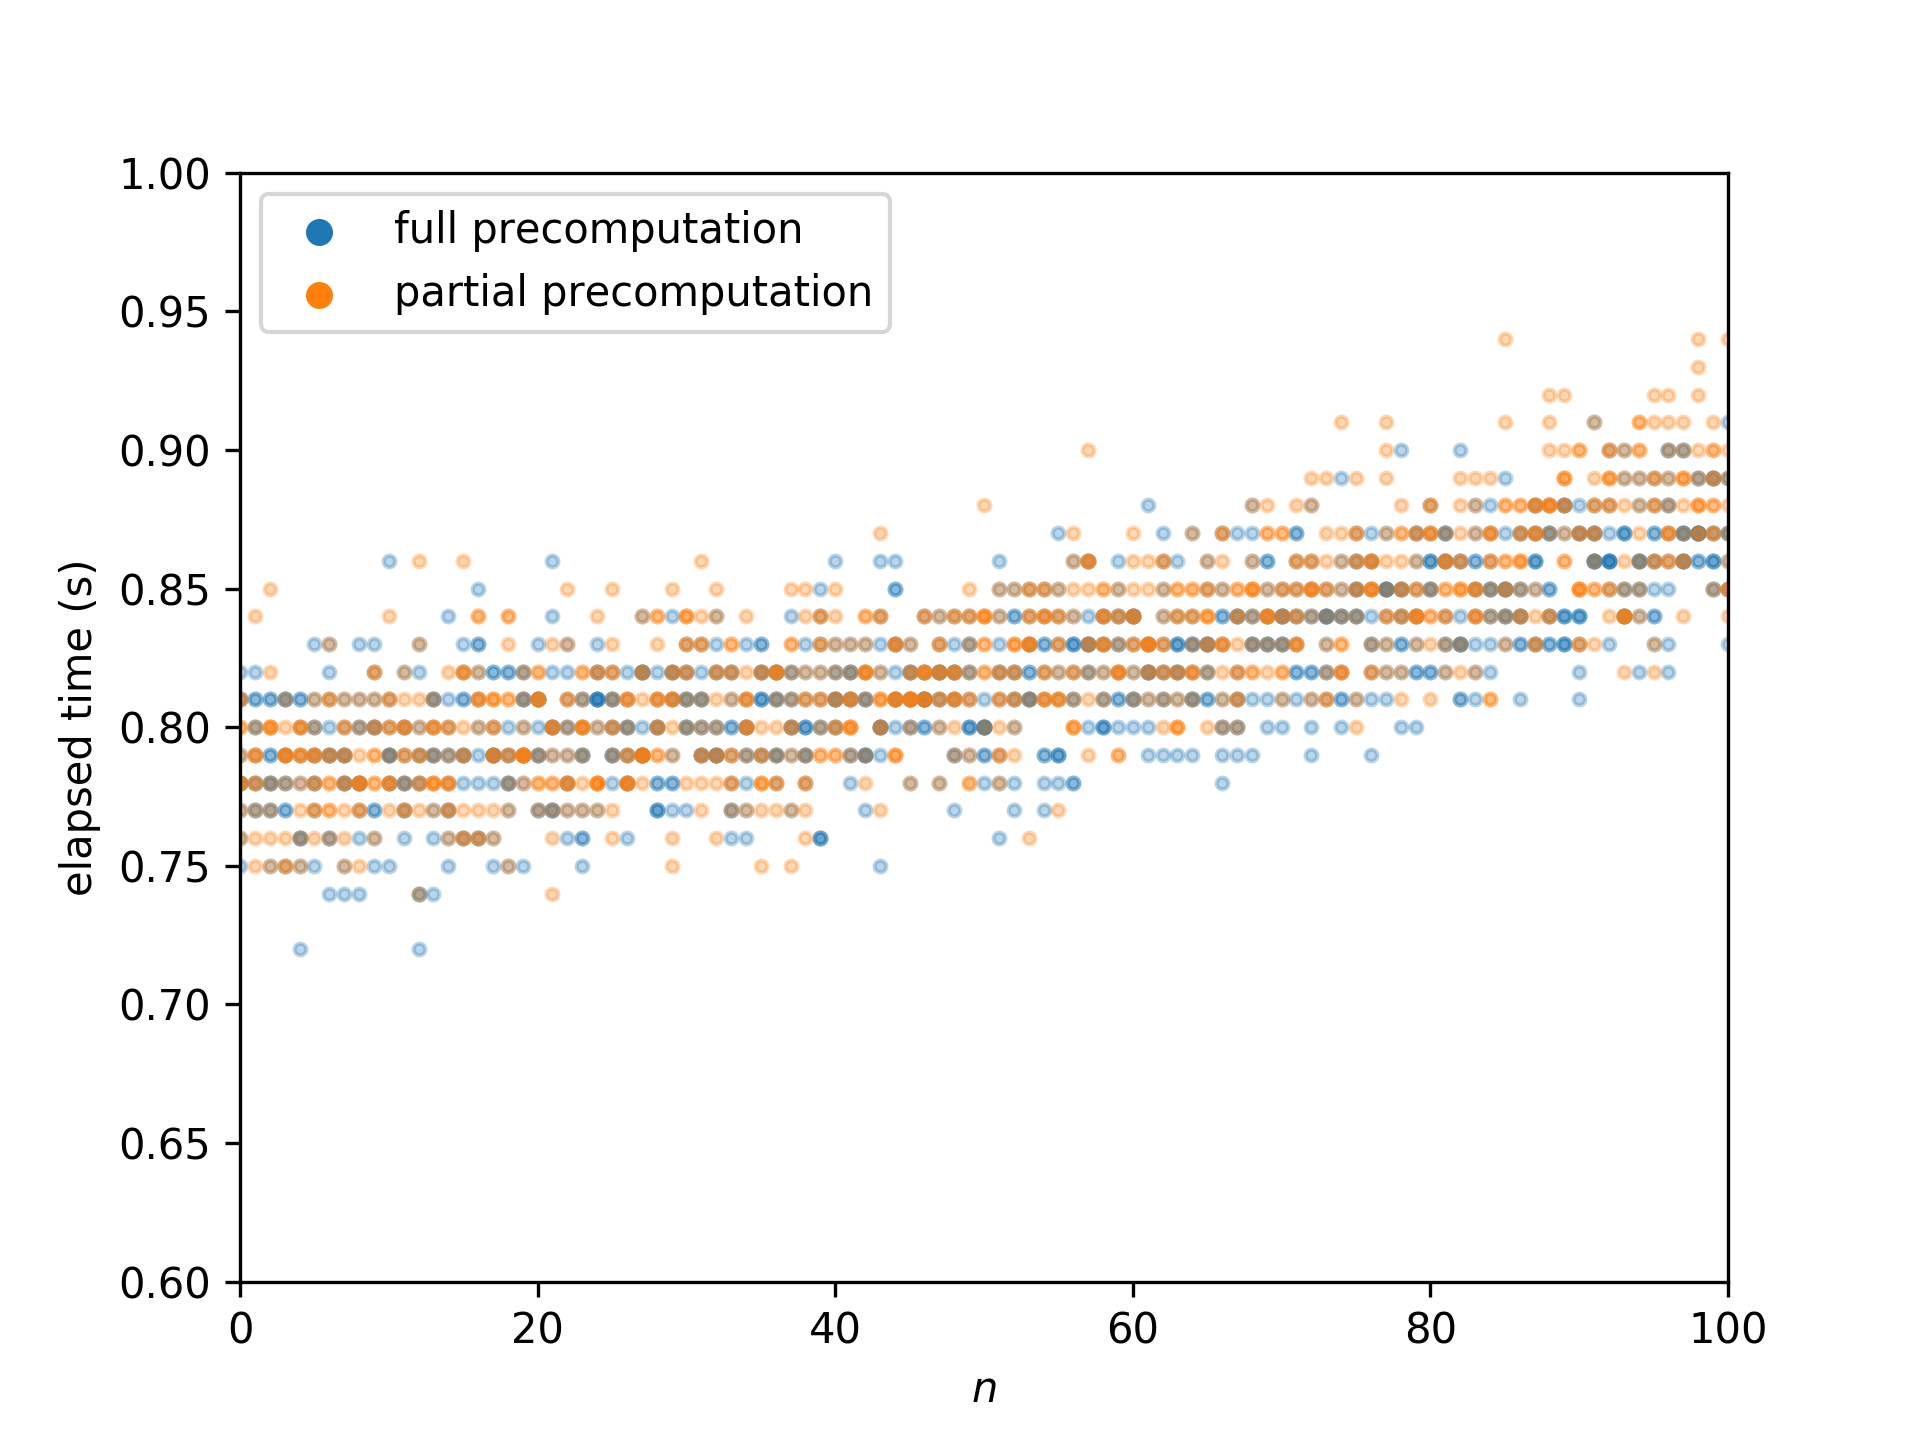
\includegraphics[scale=0.7]{figures/precomputation_cpu_small}
	\caption{Elapsed time comparison where $m=10$ and $0\leq n\leq 100$ with 1000 samples.}
\end{figure}

\begin{figure}[H]
	\centering
	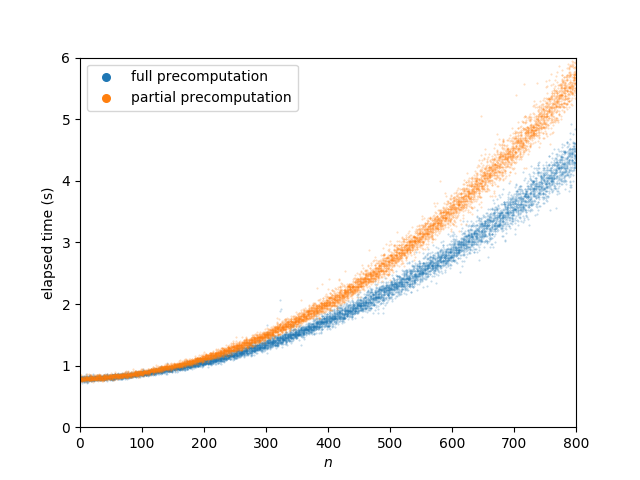
\includegraphics[scale=0.7]{figures/precomputation_cpu_big}
	\caption{Elapsed time comparison where $m=10$ and $0\leq n\leq 800$ with 8000 samples.}
\end{figure}

\begin{figure}[H]
	\centering
	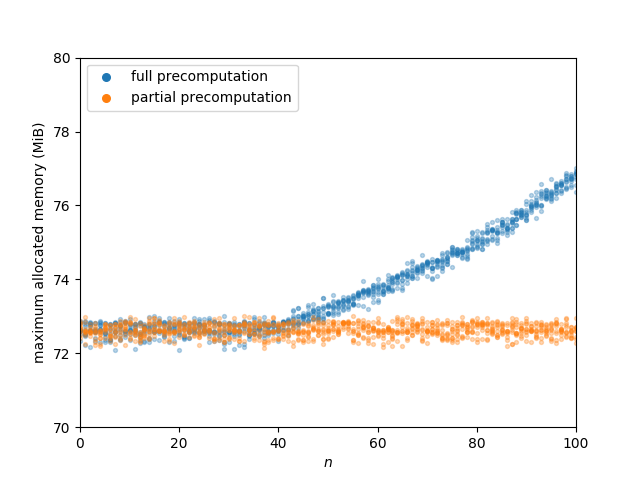
\includegraphics[scale=0.7]{figures/precomputation_memory_small}
	\caption{Maximum allocated memory comparison where $m=10$ and $0\leq n\leq 100$ with 1000 samples.}
\end{figure}

\begin{figure}[H]
	\centering
	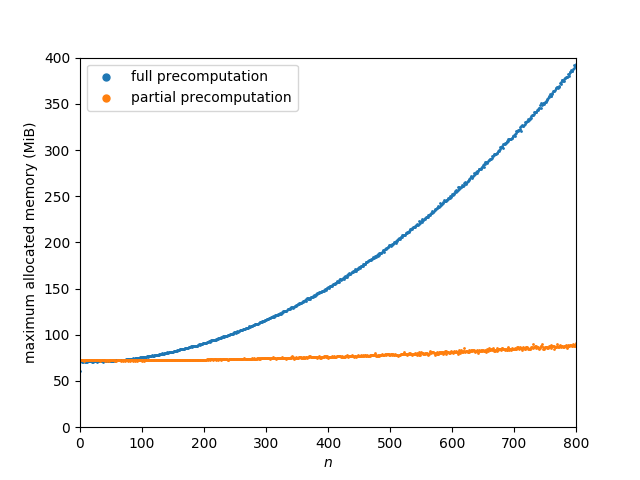
\includegraphics[scale=0.7]{figures/precomputation_memory_big}
	\caption{Maximum allocated memory comparison where $m=10$ and $0\leq n\leq 800$ with 8000 samples.}
\end{figure}

\section{Questionnaire}

We conduct surveys with three disjoint sample groups.

\begin{itemize}
	\item \textbf{Group 1}: 10 people who are not given any explanations.
	\item \textbf{Group 2}: 12 people who are given simple explanations generated from the tool, but do not have interactive access to the tool.
	\item \textbf{Group 3}: 7 people who are given interactive access to the tool.
\end{itemize}

In all groups, we used the same questionnaire, which can be found in the appendix. Each question was carefully designed to be completed mentally while exploring concepts in makespan scheduling. We do not ask about feasibility because its validation is trivial. 

\begin{itemize}
	\item Question 1 shows an efficient but non-optimal schedule. The tool does not explain optimality, so users can see cases where the tool may not be helpful.
	\item Question 2 shows a schedule with more machines and jobs, to test whether users can find improvements in a non-trivial schedule. It is possible to optimise the schedule in one single exchange, but this may not be obvious.
	\item Question 3 shows an application of fixed decisions.
	\item Question 4 explores pairs of jobs, which can be modelled using fixed decisions. The question explores how intuition can be formed using additional constraints.
	\item Question 5 explores replanning of a schedule by insertion of a new job. Clearly, trivially inserting a new job does not result in a optimal schedule. It is possible to arrange the schedule in one single exchange before insertion to achieve an optimal updated schedule.
\end{itemize}

Although these five questions do not cover the tool's complete functionality, they seek explanations that require intuition, with or without the tool. This is important in assessing how users can operate the tool in non-trivial cases. In this survey, we asked a wide demographic, from GCSE students to graduates, including people who do have little knowledge of computer science or mathematics.

\subsection{Group 1 Results}

\begin{figure}[H]
	\begin{center}
		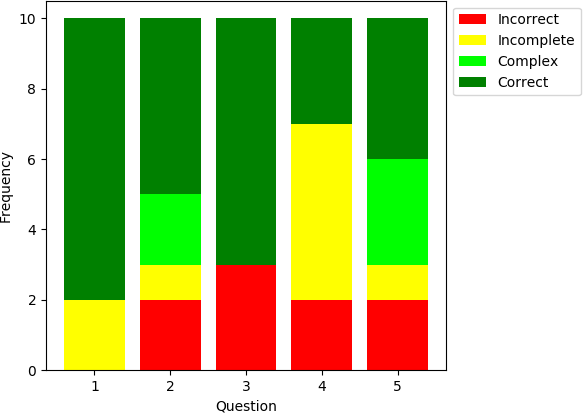
\includegraphics[scale=0.55]{figures/questionnaire_results_group_one}
	\end{center}
	\caption{Aggregated Group 1 results from Section \ref{group1data}}
	\label{group1chart}
\end{figure}

From Figure \ref{group1chart}, we see that the majority of respondents are able to get most questions correct. Some responses are considered complex, when their answers are technically correct, but give more steps than necessary. This may hint that some intuitive ways to optimise a schedule may not minimise the number of job exchanges. This was evident in Question 2 and 5, that has many jobs. We can see in more complex schedules that users give more complex answers. Some responses are considered incomplete, where only the question was partially answered. This was evident in Question 4, where many respondents failed to identity either decision yields an optimal schedule.

\subsection{Group 2 Results}

\begin{figure}[H]
	\begin{center}
		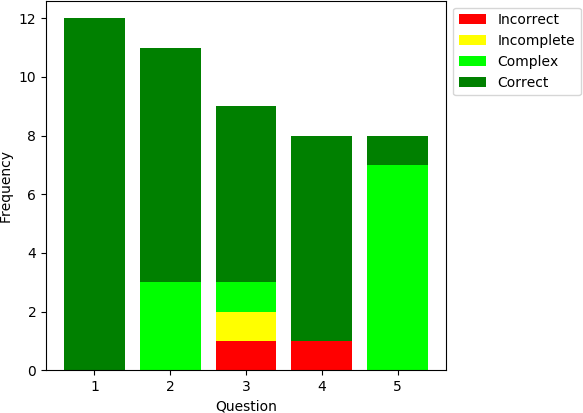
\includegraphics[scale=0.55]{figures/questionnaire_results_group_two}
	\end{center}
	\caption{Aggregated Group 2 results from Section \ref{group2data}}
	\label{group2chart}
\end{figure}

From Figure \ref{group2chart}, we can make the following observations of Group 2 compared to Group 1:
\begin{itemize}
	\item Group 2 respondents performed better than Group 1, and in less time, from 15 minutes 37 seconds to 9 minutes 12 seconds on average, excluding outliers.
	\item Group 1 respondents completed all questions, but there a few Group 2 respondents who did not answer the latter questions. This is illustrated the constant bar heights in Figure \ref{group1chart} and decreasing bar heights in Figure \ref{group2chart}.
	\item When relevant explanations are given in Questions 2 and 5, there are more complex answers in Group 2 than Group 1. The answers suggests that respondents are likely to select the easiest to understand explanation, rather than the simplest optimal schedule. This is significant in Question 5, where many respondents used the first suggestion from the explanation without further intuition.
	\item Question 3 and 4 give situations in which respondents answer which situation results in a more optimal schedule. We can see that explanations significantly improve answers.
	\item In question 1, the explanation given was not relevant, so we would expect answers from Groups 1 and 2 would be similar because the underlying question is the same. From the data, we can see some variance between Groups 1 and 2.
\end{itemize}

\subsection{Group 3 Results}

\begin{figure}[H]
	\begin{center}
		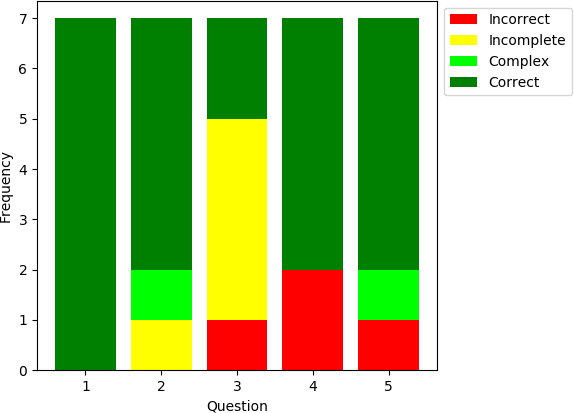
\includegraphics[scale=0.55]{figures/questionnaire_results_group_three}
	\end{center}
	\caption{Aggregated Group 3 results from Section \ref{group3data}}
	\label{group3chart}
\end{figure}

\begin{itemize}
	\item Group 3 respondents took the longest to answer the questions, with 18 minutes and 27 seconds, excluding outliers. Users spent time understanding how to use the tool. To give a more fair comparison of time, users should not been able to start the questionnaire while reading the user guide.
	\item From question 3, many respondents said to simply move jobs to satisfy negative fixed decisions, without concern of the schedule's optimality. This suggests that users took the suggestions from the took too literally. As many users suggested local changes, many answers were considered incompletes.
\end{itemize}

\subsection{Summary}

\begin{figure}[H]
	\begin{center}
		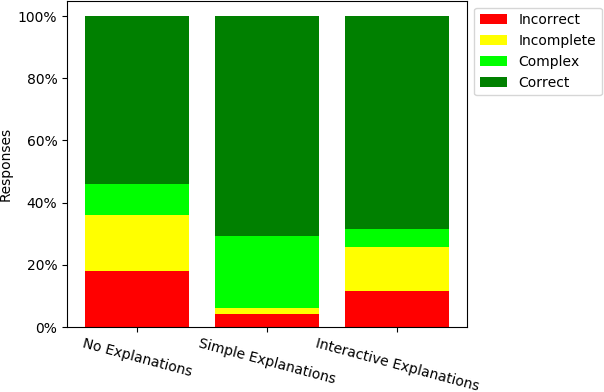
\includegraphics[scale=0.55]{figures/questionnaire_results_summary}
	\end{center}
	\caption{Aggregated results from Figures \ref{group1chart}, \ref{group2chart}, and \ref{group3chart}}
	\label{summarychart}
\end{figure}

\begin{itemize}
	\item Group 1 has the worst performance.
	\item Group 2 has the best performance, but many answers use are long and complex, often using the first obvious solution.
	\item Group 3 has the median performance, with many incomplete answers, using only one iteration of the tool.
\end{itemize}

\subsection{Feedback}

During development of the tool and questionnaires, I asked my colleagues and friends for feedback about the tool.

\begin{itemize}
	\item In early versions of the tool, the GUI did not arrange textboxes and buttons into groups such as problem, schedule and explanation. Instead, all buttons and their functionality were exposed as an menu. This was confusing to new users because it was not evident which textboxes were input or output.
	\item The paper \cite{aes} represented machine job pair assignments as a pairs of integer indices. The tool internally uses indices to compute explanations, however exposing both machines and job as integer indices was confusing. Therefore, jobs are now represented alphabetically.
	\item The tool uses regular expressions to validate user input. Many users complained about the strict validation errors. We solve this by pre-processing the input by correcting missing or surplus white-space.
\end{itemize}